\documentclass[12pt,a4paper]{article}

% ==================================================
% 1. Language and Fonts
% ==================================================
\usepackage[T1]{fontenc}
\usepackage[british]{babel}
\usepackage{csquotes}

% Use standard LaTeX fonts (comment out fontspec if not using XeLaTeX/LuaLaTeX)
% If you want to use fontspec, uncomment the lines below and ensure the font is installed
% \usepackage{fontspec}
% \setmainfont{Arial}  % or another installed font

% ==================================================
% 2. TikZ and PGFPlots (for figures)
% ==================================================
\usepackage{tikz}
\usetikzlibrary{
  shapes.geometric,
  positioning,
  fit,
  backgrounds,
  shadows,
  arrows.meta,
  calc
}

\usepackage{pgfplots}
\pgfplotsset{
  compat=1.18,
  every axis/.append style={
    cycle list name=black white
  }
}
\usepgfplotslibrary{statistics}

% Define colors for architecture diagram
\definecolor{layer1bg}{RGB}{240,248,255}
\definecolor{layer1border}{RGB}{70,130,180}
\definecolor{layer2bg}{RGB}{255,250,240}
\definecolor{layer2border}{RGB}{218,165,32}
\definecolor{layer3bg}{RGB}{240,255,240}
\definecolor{layer3border}{RGB}{60,179,113}

% Define color for feature importance bar chart
\definecolor{steelblue}{RGB}{70,130,180}

% ==================================================
% 3. Page Layout
% ==================================================
\usepackage[
  a4paper,
  margin=1.5cm
]{geometry}

\usepackage{setspace}
\singlespacing

% ==================================================
% 4. Float Control
% ==================================================
\usepackage{placeins}
\usepackage{float}

% ==================================================
% 5. Section Formatting (UNNUMBERED)
% ==================================================
\usepackage{titlesec}
\titleformat{\section}{\normalfont\Large\bfseries}{}{0em}{}
\titleformat{\subsection}{\normalfont\large\bfseries}{}{0em}{}
\titleformat{\subsubsection}{\normalfont\normalsize\bfseries}{}{0em}{}

% ==================================================
% 6. Mathematics
% ==================================================
\usepackage{amsmath}
\usepackage{amsfonts}

% ==================================================
% 6.1 Lists
% ==================================================
\usepackage{enumitem}

% ==================================================
% 7. Tables
% ==================================================
\usepackage{array}
\usepackage{tabularx}
\usepackage{booktabs}
\usepackage{longtable}
\usepackage{threeparttable}
\usepackage{adjustbox}

% ==================================================
% 8. Figures
% ==================================================
\usepackage{graphicx}
\usepackage{caption}
\usepackage{subcaption}
\usepackage{rotating}

% ==================================================
% 9. Algorithms
% ==================================================
\usepackage[ruled,vlined,linesnumbered]{algorithm2e}

% ==================================================
% 10. Bibliography — APA Style
% ==================================================
\usepackage[
  style=apa,
  backend=biber,
  uniquelist=false,
  uniquename=false
]{biblatex}
\DeclareLanguageMapping{british}{british-apa}
\addbibresource{references.bib}

% ==================================================
% 11. Hyperlinks
% ==================================================
\usepackage[colorlinks=false,pdfborder={0 0 0}]{hyperref}

% ==================================================
% Document Start
% ==================================================
\title{Beyond Attribution: A Falsifiability Framework for Reliable Credit Risk Explanations}
\author{}        % Anonymous for blind review
\date{}

\begin{document}
\maketitle

% ==================================================
% Main Content
% ==================================================

\begin{abstract}
Machine learning explanations are often treated as credible outputs of model introspection, yet they may reflect statistical artefacts rather than genuine learned patterns. This study addresses a critical gap in credit-risk governance: the need for scientifically rigorous, testable explanations rather than post-hoc narratives. We propose a falsifiability framework that treats explanations as empirical hypotheses subject to systematic validation. The framework operationalizes this through three epistemically distinct components: (1) dual-selector feature stabilization combining supervised learning with dimension reduction; (2) reliability diagnostics including sanity ratio validation and signal-to-noise discrimination; and (3) a constrained generative AI module that grounds natural language explanations in validated SHAP evidence. By integrating explanation reliability assessment directly into model development—rather than treating it as an afterthought—we demonstrate that strong predictive performance and reliable explanations are orthogonal properties requiring independent scrutiny. Our experimental validation on credit-risk datasets shows that explanations flagged as unreliable by our sanity checks correspond to models with hidden performance degradation, establishing empirical grounding for the falsifiability approach. This work enables transparent, auditable explanations suitable for regulatory compliance and stakeholder trust, fundamentally advancing how financial institutions govern machine learning systems.

\end{abstract}

\textbf{Keywords}: Credit Risk, Explainability, Reliability, Falsifiability, SHAP, Model Governance
\section{Introduction}

Credit-risk assessment plays a central role in financial decision-making, shaping lending policies and capital allocation in regulated institutions \parencite{Baesens2003_benchmarking,Lessmann2015_benchmarking}. Contemporary machine-learning models have substantially improved predictive discrimination, yet their explanations remain epistemically untested. A widespread assumption persists in practice: strong predictive performance implies reliable model explanations. This assumption is false. A model's ability to discriminate borrowers by default risk does not guarantee that its feature attributions reflect genuine learned structure rather than statistical artefacts, sampling noise, or spurious correlations \parencite{Hassija2024_interpreting}. This disconnect between prediction and explanation constitutes a fundamental scientific problem: explanations are treated as credible outputs rather than as empirical hypotheses subject to rigorous validation.

The challenge is compounded by the proliferation of post-hoc explainability tools and generative AI. SHAP and LIME assign numerical attributions to features, addressing some interpretability concerns in high-accuracy ensemble models \parencite{Ribeiro2016_why,Lundberg2017_unified}. However, growing evidence indicates that these attribution methods are highly sensitive to background distributions and sampling noise, frequently reflecting artefacts rather than genuine model structure \parencite{Slack2020_fooling,Hassija2024_interpreting}. Recent applications of generative AI that translate attribution scores into natural-language explanations remain largely unconstrained, further amplifying risks of hallucination, narrative inflation, and spurious causal claims \parencite{Hassija2024_interpreting}. The result is a proliferation of confident-sounding explanations with no mechanism to assess their empirical grounding.

This fragmentation exposes a deeper methodological gap: explainability in credit-risk modelling is rarely treated as a falsifiable scientific process. Existing work predominantly frames explanations as descriptive summaries or visualisation artefacts rather than as testable hypotheses subject to systematic evaluation. No prior framework integrates predictive modelling, attribution stability assessment, and constrained generative reasoning while explicitly quantifying whether explanatory signals persist under empirical scrutiny \parencite{Slack2020_fooling,Hassija2024_interpreting}.

This paper addresses this gap by proposing a falsifiability framework that reframes explainability from narrative generation to empirical validation. The core insight is simple but consequential: treat explanations as claims subject to reliability testing. The framework introduces three epistemically distinct components: (1) dual-selector feature stabilisation that grounds attributions in multiple signal sources prior to model training; (2) reliability diagnostics based on sanity ratio validation and signal-to-noise discrimination, enabling explicit assessment of whether attribution signals are robust or spurious; and (3) a constrained generative-AI module that produces human-readable explanations only when reliability thresholds are met, accompanied by explicit uncertainty qualifications. Rather than suppressing explanations with low reliability, the framework routes them to the generative module with uncertainty caveats, ensuring stakeholders are never presented with unfounded confidence.

To stabilise the features used for explanation, the framework adopts the Feature Selector-classifier Optimization Framework proposed by Zeng et al. \parencite{Zeng2024_ensemble}. Their dual-selector mechanism—combining nonlinear Random Forest importance with sparse L1-regularised logistic regression coefficients—establishes a stable feature foundation prior to SHAP analysis. This hybrid design reduces estimator bias while preserving both interaction-aware and linear structural signals, creating the epistemic conditions necessary for trustworthy attribution.

Using the German Credit dataset as a controlled benchmark, the framework is evaluated across a broad family of calibrated classification models to assess both predictive performance and the empirical reliability of their explanations \parencite{Baesens2003_benchmarking,Lessmann2015_benchmarking}. The results reveal a structural paradox: explanation quality varies independently of predictive accuracy, and many high-performing models produce feature attributions flagged as unreliable by sanity checks. By providing explicit, quantifiable diagnostics for explanation reliability, this work establishes a foundation for treating explainability as a scientifically testable—and falsifiable—component of model validity rather than as a cosmetic add-on. The implications extend to regulatory compliance: financial institutions can now ground model governance in transparent, auditable explanations rather than in subjective narratives.

\section{Literature Review}

Research on credit-risk modelling has evolved along three largely disconnected trajectories: optimisation of predictive algorithms, development of post-hoc interpretability methods, and, more recently, the use of generative AI for model oversight. This fragmentation has created a critical blind spot: although robust benchmarks for predictive accuracy are well established, the scientific standards for assessing explanation reliability remain underdeveloped. Methodological fragmentation persists: studies emphasising predictive discrimination often sideline interpretability altogether, while explainability-focused work frequently frames explanations as descriptive narratives rather than as testable claims. No systematic approach yet integrates explanation reliability as a first-class validation concern alongside predictive performance. This review synthesises these strands to motivate the unified predictive--explanatory framework proposed in this study, which positions explanations as empirical hypotheses subject to falsifiable testing.

\medskip
\noindent\textbf{Predictive AI Research and Feature Optimization}
Early credit-risk models relied on classical statistical techniques such as logistic regression and linear discriminant analysis, valued for transparent coefficient structures \parencite{Desai1996_credit}. However, these approaches struggle to capture nonlinear interactions and heterogeneous borrower behaviour. Comparative benchmarks, notably by Baesens et al.\ \parencite{Baesens2003_benchmarking}, consistently show that such linear assumptions underperform relative to flexible machine-learning models.

As a result, ensemble-based methods—including Random Forest, Gradient Boosting, XGBoost, and LightGBM—have become dominant in credit scoring, delivering substantial gains in discriminatory power (AUC) and separation efficiency (KS) \parencite{Lessmann2015_benchmarking, Verbraken2014_profit}. Although deep learning has been explored, evidence indicates that for modest tabular datasets such as German Credit, well-tuned tree ensembles and regularised linear models often outperform more complex architectures \parencite{Louzada2016_economics, YehLien2009_comparisons}.

Feature stability has emerged as a critical yet underemphasised determinant of both predictive and explanatory robustness. This is consequential for interpretability: if feature rankings themselves are unstable across random seeds or background distributions, then SHAP attributions computed on those features inherit that instability, rendering explanations unreliable even if the model's predictive accuracy is high. Addressing this, Zeng et al.\ \parencite{Zeng2024_ensemble} proposed a Feature Selector-classifier Optimization Framework that couples feature selection techniques (e.g., Random Forest and Logistic Regression) with ensemble classifiers. Their dual-selector approach stabilises the feature foundation before model training, reducing estimator bias while preserving both nonlinear interaction signals and sparse linear structure. This principle is critical for explanation reliability: downstream explanations built on unstable features will themselves be unstable, regardless of model accuracy. This study adopts this principle to ground downstream SHAP analysis in stable, validated predictive signals rather than in unstable single-estimator rankings.

Robustness is further shaped by the handling of class imbalance. Methods such as SMOTE can improve minority-class detection without degrading generalisation, provided they are applied strictly within stratified cross-validation to prevent information leakage \parencite{Chawla2002_smote, WangYu2025_twostage}.

\medskip
\noindent\textbf{The Interpretability Gap and the Reliability Problem}
Interpretability is a regulatory and practical requirement in credit risk. While traditional models offered intrinsic interpretability \parencite{Hand2009_hmeasure}, the opacity of modern ensemble methods has driven reliance on post-hoc attribution tools. However, this shift has created a subtle but consequential problem: interpretability (the ability to describe what a model does) has become conflated with reliability (the assurance that those descriptions are trustworthy). These are orthogonal properties.

LIME \parencite{Ribeiro2016_why} and SHAP \parencite{Lundberg2017_unified} have become standard approaches for explaining black-box models by assigning local feature attributions. These methods are commonly used to assess the economic plausibility of model drivers \parencite{WangYu2025_twostage}. However, growing evidence reveals a fundamental problem: these attribution methods produce confidence-sounding outputs regardless of whether the underlying signal is robust or noisy. Hassija et al.\ \parencite{Hassija2024_interpreting} demonstrate that attribution scores often conflate signal and noise, while Slack et al.\ \parencite{Slack2020_fooling} show that they are vulnerable to adversarial manipulation, raising concerns for regulated deployment. Critically, no standard methodology distinguishes between attributions driven by genuine learned structure and those driven by statistical artefacts.

The emergence of generative AI to translate attribution scores into natural-language explanations has amplified this problem. These approaches typically lack epistemic constraints and remain susceptible to hallucination and narrative inflation. The result is a proliferation of confident-sounding explanations with no mechanism to assess their empirical grounding. A model can achieve state-of-the-art predictive accuracy while producing feature attributions that are internally inconsistent or driven primarily by noise rather than signal—yet practitioners have few tools to detect this failure.

Crucially, no prior research integrates predictive modelling, feature-stability optimisation, and generative explanation within a unified framework that subjects explanations to explicit, rejectable reliability and signal-quality diagnostics. The field treats explainability as an interpretive challenge (how to describe predictions) rather than as a validation challenge (whether those descriptions are empirically grounded). This study addresses this gap by proposing a falsifiability framework that treats explanations not as descriptive artefacts but as claims whose reliability must be systematically tested, advancing credit-risk modelling toward a scientifically rigorous explanatory paradigm grounded in testable hypotheses rather than narrative convenience.

\section*{Methodology}

This study adopts a unified predictive--explanatory architecture grounded in falsifiability principles to benchmark credit-risk models while explicitly evaluating the reliability of their explanations. The framework integrates a calibrated predictive pipeline across multiple algorithmic families with a dual-selector feature stabilisation layer and a constrained generative explanation module. Critically, the methodology operationalizes falsifiability by embedding reliability diagnostics as quantifiable rejection conditions: explanations are suppressed when signal-to-noise discrimination indicates weak attribution evidence, and generated narratives are accompanied by explicit uncertainty qualifications. This ensures that predictive performance, attribution stability, and explanatory uncertainty are assessed within a single coherent workflow oriented toward empirical validation rather than narrative confidence.

\medskip
\noindent\textbf{Data and Preprocessing}
The experiments utilise the German Credit dataset from the UCI Machine Learning Repository \parencite{uci_german_credit}, a widely used benchmark in credit-risk research comprising 1,000 observations (700 non-default and 300 default cases) and 20 attributes \parencite{Baesens2003_benchmarking}. This dataset is chosen as a controlled benchmark precisely because of its moderate size and complexity: large enough to support ensemble learning yet small enough for thorough reliability assessment without computational barriers to exhaustive cross-validation and sanity checking.

To ensure robust model estimation and prevent confounding of predictive and explanatory reliability, the data undergo a standardised preprocessing sequence grounded in a principle of minimal assumptions: attributes with more than 90\% missing values are removed (eliminating spurious correlations from sparse data), while remaining numerical and categorical missing values are imputed using median and mode strategies, respectively. Categorical variables are transformed using one-hot encoding, and numerical features are standardised to zero mean and unit variance. This conservative preprocessing preserves data structure without introducing artificial associations that could confound downstream SHAP analysis.

Class imbalance is addressed using the Synthetic Minority Over-sampling Technique (SMOTE), applied strictly within the training folds of stratified cross-validation. This placement is critical: applying SMOTE before splitting would contaminate test-set evaluations with synthetic data, undermining the empirical validation of both predictive performance and explanation reliability. By applying SMOTE only to training folds, we ensure that performance estimates and reliability diagnostics reflect genuine generalisation rather than artefacts of resampling \parencite{Chawla2002_smote, WangYu2025_twostage}.

\medskip
\noindent\textbf{Predictive Modelling Framework}
The unit of analysis is the \emph{model family}, interpreted as a functional constructor that defines a class of predictive algorithms sharing a common architectural principle. Four primary model families are evaluated: Linear Models, Boosting, Bagging, and Instance-Based Learners. Hyperparameter choices (e.g., ensemble size, learning rate, regularisation structure, distance weighting) represent implementation variants of the same constructor and are not treated as independent hypotheses, but rather as necessary operational specifications that instantiate the family's functional definition.

To establish a comprehensive baseline that adequately exercises each family's representational capacity, 75 calibrated model configurations are systematically evaluated across these families, with the configuration space summarised in Table~\ref{tab:classification_models}. This sampling strategy ensures that each model family is assessed fairly by exploring its operationally relevant hyperparameter ranges. All models are trained within a stratified cross-validation framework and calibrated using \texttt{CalibratedClassifierCV} to ensure that predicted scores correspond to well-formed probability estimates, a prerequisite for meaningful risk ranking and expected-loss interpretation.

%**********************Table: Classification Models***********************
\begin{table}[ht]
\centering
\caption{Model families as functional constructors and their implementation variant dimensions. Hyperparameters specify operational instantiations of each family's architectural principle rather than independent competing hypotheses.}
\label{tab:classification_models}
\begin{tabularx}{\textwidth}{p{2.5cm} X r}
\toprule
\textbf{Model Family} & \textbf{Constructor Implementation Dimensions (hyperparameter variants)} & \textbf{Configurations} \\
\midrule
Linear & Solver and regularisation structure in logistic regression (lbfgs, saga, newton-cg; L1, L2, ElasticNet) & 6 \\
\midrule
Boosting & Ensemble size and learning rate for decision-stump AdaBoost, plus ensemble size for stochastic gradient boosting & 28 \\
\midrule
Bagging & Ensemble size for bagged trees and neural networks; ensemble size and feature subsampling for random forests & 36 \\
\midrule
Instance-Based & Neighbourhood size and distance weighting in $k$-NN, with one cross-validated tuned model & 5 \\
\midrule
\textbf{Total Configurations} & \textbf{Combined instantiations across all constructors} & \textbf{75} \\
\bottomrule
\end{tabularx}
\end{table}

\medskip
\noindent\textbf{Unit of Analysis: Model Families as Functional Constructors}
A critical conceptual distinction underlies the experimental design and the falsifiability framework: the unit of analysis is \emph{not} the individual trained model with specific hyperparameter values, but the \emph{model family itself}, understood as a functional constructor that encodes an algorithmic principle. This distinction matters for reliability assessment. Hyperparameter choices (ensemble size, learning rate, regularisation magnitude) do not constitute independent competing hypotheses; instead, they represent operational implementation variants necessary to instantiate the constructor's functional definition. For example, varying ensemble size in a Bagging constructor does not generate a distinct hypothesis but rather explores how the bagging principle scales across different operational regimes. Similarly, varying regularisation in logistic regression does not test whether regularisation is correct—it tests how much regularisation best instantiates the linear-classification principle for this particular dataset.

This interpretation ensures that comparative assessment is conducted at the appropriate level of abstraction: families are compared as distinct algorithmic approaches, while within-family variation documents the family's effective operating envelope and operational constraints. The selection of best instantiation within each family identifies the most effective realisation of that family's core architectural principle. Crucially, this design prevents confusing poor hyperparameter choices with fundamental algorithmic failure: when an explanation is flagged as unreliable, we ask whether the reliability problem is intrinsic to the family's principle or contingent on suboptimal instantiation.

\medskip
\noindent\textbf{Unified Predictive and Explanatory Architecture}
The framework is organised into three epistemically distinct layers that define what tasks are permissible, how information flows, and what constraints apply. These layers establish \emph{architectural principles} that any valid instantiation must respect: feature stabilisation must precede model training, model selection must be comparative across families, and explanation generation must be constrained by reliability diagnostics. This abstract architecture, illustrated in Figure~\ref{fig:architecture}, is independent of implementation details and does not itself specify execution order, selection thresholds, or failure modes.

\medskip
\noindent\textbf{Operational Workflow and Instantiation}
The architecture is instantiated through a concrete operational procedure that specifies the \emph{exact sequencing, selection criteria, and failure conditions} under which a valid model and explanation are produced. This procedure is summarised in Algorithm~\ref{algo:full_pipeline}. Unlike the architecture, the workflow is falsifiable: it specifies quantitative selection criteria (AUC maximisation), computational order (feature stabilisation before model training), and explicit rejection conditions (explanation suppression when Sanity Ratio indicates weak signal). The algorithm is auditable—a reader can verify whether an implementation adheres to it by inspecting computational logs and decision records.

%*********************Algorithm: Operational Workflow*********************
\begin{algorithm}[H]
\caption{Operational Instantiation: Unified Predictive and Explanatory Workflow}
\label{algo:full_pipeline}

\KwIn{Dataset $D$, Model Registry $\mathcal{M}$, Configuration Set $\mathcal{C}$}
\KwOut{Benchmark Model $B^*$, Explanations $E$, Reliability Diagnostics $D_{rel}$}

\textbf{Phase 1: Feature Screening (Dual-Selector)}\\
Train Random Forest and L1-logistic regression; obtain importance scores $Imp_{RF}$ and $Imp_{L1}$.\\
Compute composite score: $I_c = \frac{1}{2}(\mathrm{norm}(Imp_{RF}) + \mathrm{norm}(Imp_{L1}))$.\\
Rank features by $I_c$; apply domain-based exclusion rationale; select screened feature set.\\

\textbf{Phase 2: Model Training and Selection}\\
\For{each model family $F \in \mathcal{M}$}{
  Perform stratified split; apply SMOTE; train calibrated instantiations; evaluate AUC.
}
Define benchmark: $B^* = \arg\max_{B_F}(\mathrm{AUC})$.\\

\textbf{Phase 3: Explainability and Reliability}\\
Compute SHAP values (global and local) for $B^*$.\\
Evaluate stability via reliability diagnostics; compute Sanity Ratio $\rho$.\\
\If{$\rho < 0.95$}{
  Generate explanation with uncertainty caveats\;
}
\Else{
  Generate high-confidence explanation\;
}

\textbf{Phase 4: Constrained Generative Explanation}\\
\If{Reliability Diagnostics indicate signal $\ge$ noise}{
  Extract top-$k$ SHAP features; construct structured prompt (feature names, values, SHAP contributions, prediction, label)\;
  Invoke LLM to generate two-segment explanation with constraint: ground narrative in validated SHAP evidence\;
}
\Else{
  Flag explanation as unreliable; suppress confident claims\;
}
\Return{$B^*, E, D_{rel}$}

\end{algorithm}

\medskip
\noindent\textbf{Generative AI Explanation Layer}

To enhance communicability without compromising epistemic rigor, we employ a constrained generative AI module that translates validated SHAP evidence into natural-language explanations. Unlike unconstrained narrative-generation systems, this module operates strictly within the boundaries imposed by reliability diagnostics: it may summarise evidence and articulate the reasoning implied by validated attributions, but it is not permitted to introduce causal claims, speculative associations, or narrative elements that lack empirical support. Explanation generation is suppressed entirely when reliability diagnostics indicate that attribution signals are weak relative to noise, ensuring that narrative confidence never exceeds evidential support.

The module's configuration, inputs, processing logic, and constraints are summarised in Table~\ref{tab:llm_explanation_layer}. The module receives ranked SHAP outputs, feature names, feature values, and true labels as inputs, identifying the top contributing features ordered by absolute SHAP magnitude. The LLM is constrained to operate as a machine-learning analyst, producing two short paragraphs: one explaining why the model made the prediction and another comparing the prediction to the actual outcome. This structured design ensures that generated explanations remain grounded in quantitative attribution evidence while supporting human interpretability.

\begin{table}[H]
\centering
\caption{LLM-based SHAP explanation module: configuration and constraints.}
\label{tab:llm_explanation_layer}
\footnotesize
\setlength{\tabcolsep}{4pt}
\renewcommand{\arraystretch}{1.1}
\begin{tabular}{
  >{\raggedright\arraybackslash}p{3.0cm}
  >{\raggedright\arraybackslash}p{10.8cm}
}
\toprule
\textbf{Component} & \textbf{Description} \\
\midrule
Purpose &
Generates natural-language explanations for SHAP outputs constrained by reliability diagnostics \\
\midrule
Input &
SHAP values, feature names, feature values, true label, predicted probability \\
\midrule
Processing &
Sorts features by absolute SHAP magnitude; selects top validated features for narrative \\
\midrule
Prompt Structure &
System prompt constrains LLM role as ML analyst; user prompt provides numerical context (SHAP values, predictions); required output: two short paragraphs (1) Why model predicted this outcome, (2) Prediction alignment with actual label \\
\midrule
Output &
Two paragraphs summarising SHAP-driven reasoning and prediction correctness \\
\midrule
Critical Constraint &
Narrative must remain grounded in validated SHAP evidence; no unsupported causal claims; explanation suppressed if signal \textless\, noise \\
\bottomrule
\end{tabular}
\end{table}

\medskip
\noindent\textbf{Architectural Principles: Conceptual Foundation}
The three-layer architecture below is a \emph{non-procedural} representation of task decomposition and information dependencies. It specifies what transformations are logically necessary and how information must flow between stages, but does not impose ordering constraints, quantitative selection criteria, or conditional rejection logic. Any valid instantiation must respect the architectural constraints (e.g., feature stabilisation logically precedes model training), but the specific operational realisation—including hyperparameter selection, decision thresholds, and failure handling—is determined by the algorithm.

%**********************Figure: Conceptual Architecture***********************
\begin{figure}[H]
    \centering

    \resizebox{\textwidth}{!}{%
    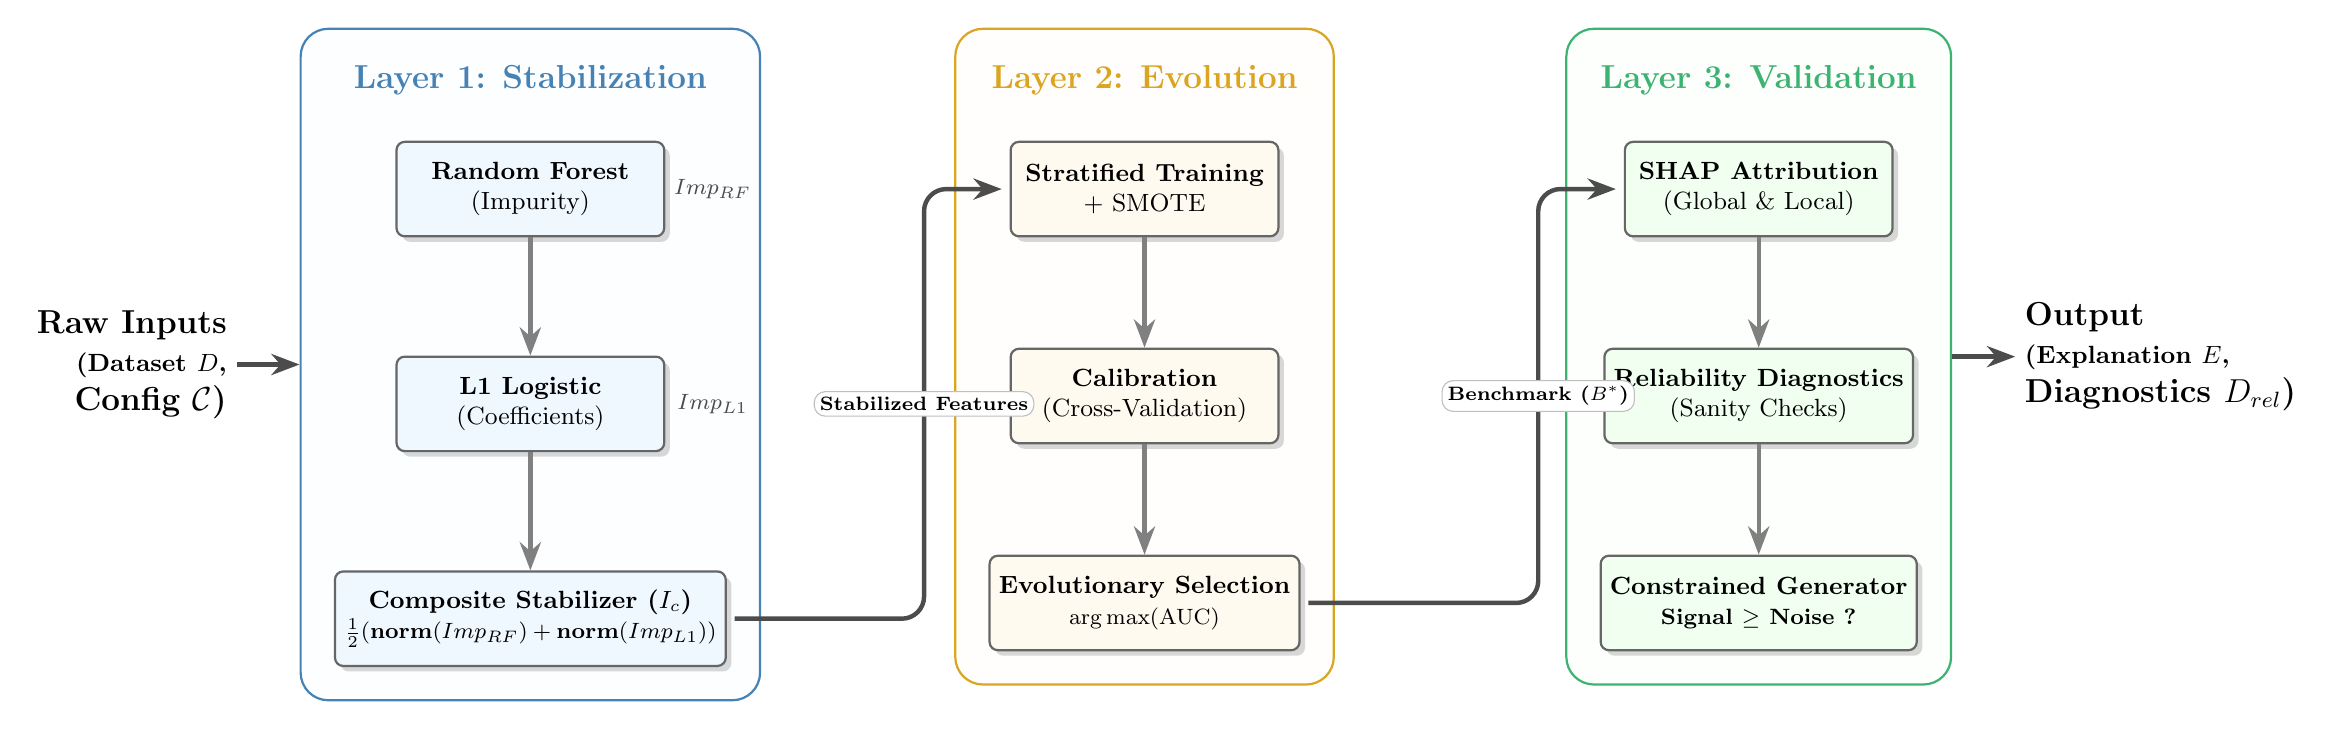
\begin{tikzpicture}[
      font=\sffamily,
      >=Stealth,
      component/.style={
        rectangle,
        rounded corners=3pt,
        draw=black!60,
        fill=white,
        thick,
        minimum height=1.2cm,
        minimum width=3.4cm,
        align=center,
        drop shadow={opacity=0.3,shadow xshift=2pt,shadow yshift=-2pt},
        font=\small\bfseries
      },
      logic/.style={
        draw=none,
        font=\footnotesize\itshape\color{black!70}
      },
      layer/.style={
        rectangle,
        rounded corners=10pt,
        draw,
        thick,
        inner sep=12pt
      },
      layerlabel/.style={
        font=\bfseries\large,
        anchor=north,
        yshift=-10pt
      },
      flow/.style={
        ->,
        ultra thick,
        black!70,
        rounded corners=8pt
      },
      arrowlabel/.style={
        fill=white,
        draw=gray!50,
        rounded corners,
        font=\scriptsize\bfseries,
        inner sep=2pt
      }
    ]

    % Coordinates
    \coordinate (col1) at (0,0);
    \coordinate (route12) at (5.0,0);
    \coordinate (col2) at (7.8,0);
    \coordinate (route23) at (12.8,0);
    \coordinate (col3) at (15.6,0);

    % Layer 1: Stabilization
    \node[component, fill=layer1bg] (rf) at ($(col1)+(0,2.8)$)
      {Random Forest\\ \normalfont (Impurity)};
    \node[component, fill=layer1bg, below=1.5cm of rf] (l1)
      {L1 Logistic\\ \normalfont (Coefficients)};
    \node[component, fill=layer1bg, below=1.5cm of l1] (composite)
      {Composite Stabilizer ($I_c$)\\
       \footnotesize $\tfrac12(\text{norm}(Imp_{RF})+\text{norm}(Imp_{L1}))$};

    \node[logic] at ($(rf.east)+(6mm,0)$) {$Imp_{RF}$};
    \node[logic] at ($(l1.east)+(6mm,0)$) {$Imp_{L1}$};

    \draw[flow,gray] (rf) -- (l1);
    \draw[flow,gray] (l1) -- (composite);

    \coordinate (layer1title) at ($(rf.north)+(0,10mm)$);
    \begin{scope}[on background layer]
      \node[layer,draw=layer1border,fill=layer1bg!20,
            fit=(layer1title)(rf)(l1)(composite)] (layer1) {};
      \node[layerlabel,text=layer1border] at (layer1.north)
        {Layer 1: Stabilization};
    \end{scope}

    % Layer 2: Evolution
    \node[component, fill=layer2bg] (training) at ($(col2)+(0,2.8)$)
      {Stratified Training\\ \normalfont + SMOTE};
    \node[component, fill=layer2bg, below=1.4cm of training] (calibration)
      {Calibration\\ \normalfont (Cross-Validation)};
    \node[component, fill=layer2bg, below=1.4cm of calibration] (selection)
      {Evolutionary Selection\\ \footnotesize $\arg\max(\mathrm{AUC})$};

    \draw[flow,gray] (training) -- (calibration);
    \draw[flow,gray] (calibration) -- (selection);

    \coordinate (layer2title) at ($(training.north)+(0,10mm)$);
    \begin{scope}[on background layer]
      \node[layer,draw=layer2border,fill=layer2bg!20,
            fit=(layer2title)(training)(calibration)(selection)] (layer2) {};
      \node[layerlabel,text=layer2border] at (layer2.north)
        {Layer 2: Evolution};
    \end{scope}

    % Layer 3: Validation
    \node[component, fill=layer3bg] (shap) at ($(col3)+(0,2.8)$)
      {SHAP Attribution\\ \normalfont (Global \& Local)};
    \node[component, fill=layer3bg, below=1.4cm of shap] (diagnostics)
      {Reliability Diagnostics\\ \normalfont (Sanity Checks)};
    \node[component, fill=layer3bg, below=1.4cm of diagnostics] (generator)
      {Constrained Generator\\ \footnotesize Signal $\ge$ Noise ?};

    \draw[flow,gray] (shap) -- (diagnostics);
    \draw[flow,gray] (diagnostics) -- (generator);

    \coordinate (layer3title) at ($(shap.north)+(0,10mm)$);
    \begin{scope}[on background layer]
      \node[layer,draw=layer3border,fill=layer3bg!20,
            fit=(layer3title)(shap)(diagnostics)(generator)] (layer3) {};
      \node[layerlabel,text=layer3border] at (layer3.north)
        {Layer 3: Validation};
    \end{scope}

    % Routing
    \coordinate (port1) at ($(composite.east)+(0.1,0)$);
    \coordinate (port2) at ($(training.west)+(-0.1,0)$);

    \draw[flow] (port1) -- (route12 |- port1) -- (route12 |- port2) -- (port2);
    \node[arrowlabel] at ($(route12 |- port1)!0.5!(route12 |- port2)$)
      {Stabilized Features};

    \coordinate (port3) at ($(selection.east)+(0.1,0)$);
    \coordinate (port4) at ($(shap.west)+(-0.1,0)$);

    \draw[flow] (port3) -- (route23 |- port3) -- (route23 |- port4) -- (port4);
    \node[arrowlabel] at ($(route23 |- port3)!0.5!(route23 |- port4)$)
      {Benchmark ($B^*$)};

    % Inputs/Outputs
    \node[left=0.8cm of layer1,align=right,font=\bfseries\large] (inputs)
      {Raw Inputs\\ \small (Dataset $D$,\\ Config $\mathcal C$)};
    \draw[flow] (inputs) -- (layer1.west);

    \node[right=0.8cm of layer3,align=left,font=\bfseries\large] (outputs)
      {Output\\ \small (Explanation $E$,\\ Diagnostics $D_{rel}$)};
    \draw[flow] (layer3.east) -- (outputs);

    \end{tikzpicture}
    }

    \caption{Conceptual Architecture: Task Decomposition and Information Constraints. This figure depicts the three foundational layers that define permissible transformations and information dependencies, independent of execution order or selection criteria. Layer 1 (Stabilization) establishes that feature importance must integrate multiple signal sources before model training. Layer 2 (Evolution) establishes that model selection occurs within a constrained family-based comparative framework. Layer 3 (Validation) establishes that explanations remain subject to signal-quality constraints and may be suppressed if diagnostics indicate unreliable attribution. The figure is non-procedural: it specifies \emph{what tasks must occur and how information is constrained}, not the sequence, decision thresholds, or failure modes that govern their instantiation. The concrete instantiation is specified in Algorithm~\ref{algo:full_pipeline}.}
    \label{fig:architecture}
\end{figure}

\FloatBarrier

\medskip
\noindent\textbf{Canonical Model Instantiation and Selection Rationale}
Rather than evaluate all hyperparameter configurations exhaustively, a single canonical instantiation is selected per family based on theoretical and structural principles. This approach ensures that comparative assessment reflects genuine algorithmic differences rather than configuration-specific tuning effects. The following canonical instantiations represent each family's core architectural principle.

\emph{Linear Models} are instantiated through two complementary variants. Unregularised logistic regression with the newton-cg solver provides the classical statistical baseline, eschewing explicit complexity penalties to preserve the foundational logistic model. Regularised logistic regression with L1-penalty via liblinear represents the modern variant that intrinsically enforces sparsity, automatically excluding irrelevant features through the penalty mechanism.

\emph{Boosting} is represented by AdaBoost with decision stumps (ensemble size 30). This instantiation embodies the original boosting principle grounded in iterative error correction. The shallow base learner (one-level decision tree) ensures theoretical clarity and computational transparency, avoiding the confounding effects of deeper trees or more complex base learners.

\emph{Bagging (CART)} employs bagged decision trees with ensemble size 500, instantiating classical bootstrap aggregation without feature subsampling. This configuration establishes the baseline ensemble principle, serving as a reference point for understanding the effects of feature subsampling introduced in Random Forest variants.

\emph{Bagging (Neural Network)} extends the bagging principle to flexible nonlinear function approximators. Bagged neural networks with ensemble size 100 represent the intersection of modern deep-learning architectures with classical ensemble methodology, demonstrating how bagging performs when applied to highly flexible learners rather than tree-based models.

\emph{Random Forest} instantiation employs $\sqrt{p}$ feature subsampling (ensemble size 500), representing a specialised variant that introduces controlled feature randomness. This configuration represents a key theoretical contribution to ensemble learning, trading reduced per-tree correlation for improvements in generalisation through feature decorrelation.

\emph{Stochastic Gradient Boosting} (ensemble size 50, learning rate 0.1) instantiates the gradient-boosting principle with conservative operational parameters. The modest ensemble scale and conservative learning rate reflect a balanced approach that prioritises approximation quality and generalisation stability over aggressive boosting.

\emph{Instance-Based} methods are represented by k-NN with $k=11$ and uniform distance weighting. This neighbourhood size balances local responsiveness (small $k$ overfit to individual observations) against global smoothing (large $k$ ignore local structure), establishing the non-parametric neighbourhood principle at an intermediate operational point.

Performance metrics for these canonical representatives are reported in Table~\ref{tab:benchmark_german_credit_record_csv}.

\medskip
\noindent\textbf{Explainability and Evaluation Architecture: Falsifiability in Practice}
The framework extends beyond predictive benchmarking by embedding explanation reliability assessment directly into the evaluation pipeline as a testable, rejectable component. Rather than treating feature attributions as self-validating artefacts, explanations are interpreted as empirical claims whose credibility depends on the empirically measured stability and strength of the underlying signal. This operationalizes falsifiability: explanations are not suppressed as failures but are explicitly subjected to signal-quality tests, with rejection conditions specified in advance (sanity ratio thresholds, noise discrimination criteria). Explanations that pass validation are accompanied by confidence metrics; those that fail validation are routed to the generative module with uncertainty caveats, creating a transparent audit trail of explanatory confidence.

\medskip
\noindent\textbf{Feature Attribution and Generative Explanation: Stabilizing Explanatory Evidence}
To mitigate instability associated with single-method feature selection and prevent attribution uncertainty from being misattributed to true signal loss, a dual-selector mechanism is employed. By combining impurity-based Random Forest importance (which captures nonlinear interactions and heterogeneous effects) with coefficient-based L1-regularised logistic regression importance (which enforces sparse, interpretable linear structure), the framework preserves both interaction-aware and linear structural signals. This dual approach grounds subsequent SHAP analysis in stable feature foundations rather than in unstable single-estimator rankings. SHAP values are then computed on this stabilised feature set and passed to a generative module that translates quantitative attributions into human-readable narratives. Critically, the generative component is constrained by the reliability diagnostics: confident explanations are produced only when sanity-ratio and signal-to-noise tests pass, preventing the LLM from generating confident narratives when underlying attribution signals are weak.

\medskip
\noindent\textbf{Evaluation Metrics}

Model evaluation in credit-risk modelling requires multidimensional assessment reflecting both regulatory requirements and practical decision-making demands. We employ a suite of complementary metrics that jointly capture discrimination, calibration, and cost-sensitive performance, as summarised in Table~\ref{tab:evaluation_metrics}.

\begin{table}[H]
\centering
\caption{Evaluation metrics for model assessment and selection.}
\label{tab:evaluation_metrics}
\small
\setlength{\tabcolsep}{4pt}
\renewcommand{\arraystretch}{1.4}
\begin{tabular}{p{1.8cm}p{2.2cm}p{3.8cm}p{4.2cm}}
\toprule
\textbf{Metric} & \textbf{Category} & \textbf{Purpose} & \textbf{Formula} \\
\midrule
AUC & Discrimination & Rank-ordering ability; threshold-independent & $\displaystyle \int_0^1 \mathrm{TPR}(x)\, d(\mathrm{FPR}(x))$ \\
KS & Discrimination & Maximum class separation & $\displaystyle \max_{t} |\mathrm{TPR}(t) - \mathrm{FPR}(t)|$ \\
\midrule
BS & Calibration & Probability calibration error & $\displaystyle \frac{1}{N} \sum_{i=1}^N (p_i - y_i)^2$ \\
\midrule
PCC & Classification & Overall accuracy & $\displaystyle \frac{\mathrm{TP} + \mathrm{TN}}{\mathrm{TP} + \mathrm{FP} + \mathrm{TN} + \mathrm{FN}}$ \\
Recall & Classification & Sensitivity; detect defaults & $\displaystyle \frac{\mathrm{TP}}{\mathrm{TP} + \mathrm{FN}}$ \\
H & Utility & Cost-sensitive performance \parencite{Hand2009_hmeasure} & $\displaystyle 1 - \frac{\mathrm{EMC}}{\mathrm{EMC}_0}$ \\
\bottomrule
\end{tabular}
\end{table}

\medskip
\noindent\textbf{Primary Selection Criterion: Discrimination as Necessary but Not Sufficient}
AUC serves as the primary model selection metric, chosen not for its optimality but for its falsifiability properties. AUC measures discriminatory power—the model's ability to rank-order observations by risk—independent of decision thresholds, providing a metric that is robust to class imbalance and threshold selection artifacts. This threshold-independence is critical for fair comparison across heterogeneous model families and enables reproducible selection logic.

However, AUC alone does not characterize explanatory reliability. The Brier Score complements AUC by quantifying probability calibration quality, measuring whether predicted default probabilities align with empirical frequencies across the full probability spectrum. Calibration and discrimination are orthogonal properties: a model can discriminate perfectly (rank order) while assigning poorly calibrated probabilities, or vice versa. By tracking both, we create the conditions for falsifying the claim that "high AUC implies reliable explanations." If a model achieves high AUC but low Brier Score, we expect its feature attributions to exhibit anomalies under sanity checking.

All metrics are computed within stratified cross-validation to ensure that performance estimates reflect genuine generalisation rather than training-set artifacts. Secondary metrics (KS, H-measure, Recall) provide diagnostic insight into separation stability, decision utility, and default-detection capability. The full metric suite creates a multi-dimensional performance space in which no single model dominates all dimensions, forcing practitioners to make trade-off choices and preventing false claims of universal optimality.

\FloatBarrier

\section*{Results}
This section reports the empirical findings of the proposed predictive--explanatory framework, organised to distinguish between predictive performance, feature importance, and explanatory reliability.
\smallskip
\noindent\textbf{Supervised Feature Importance Analysis}
Feature relevance is assessed using the proposed dual-selector mechanism, which combines Random Forest impurity-based importance with coefficient magnitudes from L1-regularised logistic regression. The aggregated feature rankings produced by the dual-selector mechanism are reported in Table~\ref{tab:fi_merged_german_credit_record}. Several key patterns emerge from the analysis.

Transaction structure emerges as the dominant driver of credit risk. Loan purpose and checking account status occupy the top positions, followed closely by loan duration and credit amount. These variables characterise the fundamental structure and terms of the transaction, suggesting that the nature and scope of the credit request are central to default risk assessment.
\smallskip

Financial capacity indicators demonstrate substantially greater predictive importance than demographic attributes. Savings status and credit history rank significantly higher than borrower age or personal characteristics, indicating that established financial behaviour and accumulated resources provide stronger signals of creditworthiness than static demographic properties. This finding aligns with established credit-risk theory, which emphasises the primacy of financial position over personal circumstances.
\smallskip

Behavioural history proves more informative than employment stability. Credit history substantially outweighs employment tenure in explaining risk, revealing that a borrower's track record of credit management carries greater explanatory power than tenure in current employment. This pattern underscores the importance of demonstrated financial discipline across the credit lifecycle.
\smallskip

Social indicators contribute minimally to discriminative power. Variables such as foreign worker status, telephone ownership, and residential stability add negligible incremental signal beyond the stronger indicators already identified. These low-impact features are subsequently excluded from the modelling phase, reducing input dimensionality without meaningful loss of predictive information.

%**********************Table and Chart: Feature Importance***********************
\begin{figure}[H]
\centering
\begin{minipage}[c]{0.48\textwidth}
\centering
\scriptsize
\begin{tabular}{@{}r l r r r@{}}
\toprule
Rank & Feature & RF Imp. & LR Coef. & Avg. \\
\midrule
1  & purpose & 0.075 & 3.884 & 0.773 \\
2  & checking\_status & 0.131 & 1.849 & 0.738 \\
3  & savings\_status & 0.065 & 2.347 & 0.534 \\
4  & months\_duration & 0.076 & 1.983 & 0.530 \\
5  & credit\_amount & 0.090 & 1.386 & 0.511 \\
6  & credit\_history & 0.065 & 1.491 & 0.424 \\
7  & employment\_since & 0.061 & 1.300 & 0.384 \\
8  & property & 0.057 & 1.026 & 0.332 \\
9  & age & 0.073 & 0.415 & 0.316 \\
10 & personal\_status\_sex & 0.045 & 1.010 & 0.282 \\
11 & other\_install\_plans & 0.042 & 0.823 & 0.244 \\
12 & housing & 0.032 & 1.050 & 0.233 \\
13 & installment\_rate & 0.034 & 0.756 & 0.204 \\
14 & foreign\_worker & 0.008 & 1.111 & 0.143 \\
15 & job & 0.041 & 0.047 & 0.140 \\
16 & existing\_credits & 0.018 & 0.720 & 0.133 \\
17 & telephone & 0.026 & 0.399 & 0.124 \\
18 & residence\_since & 0.032 & 0.000 & 0.098 \\
19 & other\_debtors & 0.020 & 0.276 & 0.086 \\
20 & people\_liable & 0.011 & 0.187 & 0.038 \\
\bottomrule
\end{tabular}
\captionof{table}{Top features by combined RF/LR importance}
\label{tab:fi_merged_german_credit_record}
\end{minipage}%
\hfill
\begin{minipage}[c]{0.50\textwidth}
\centering
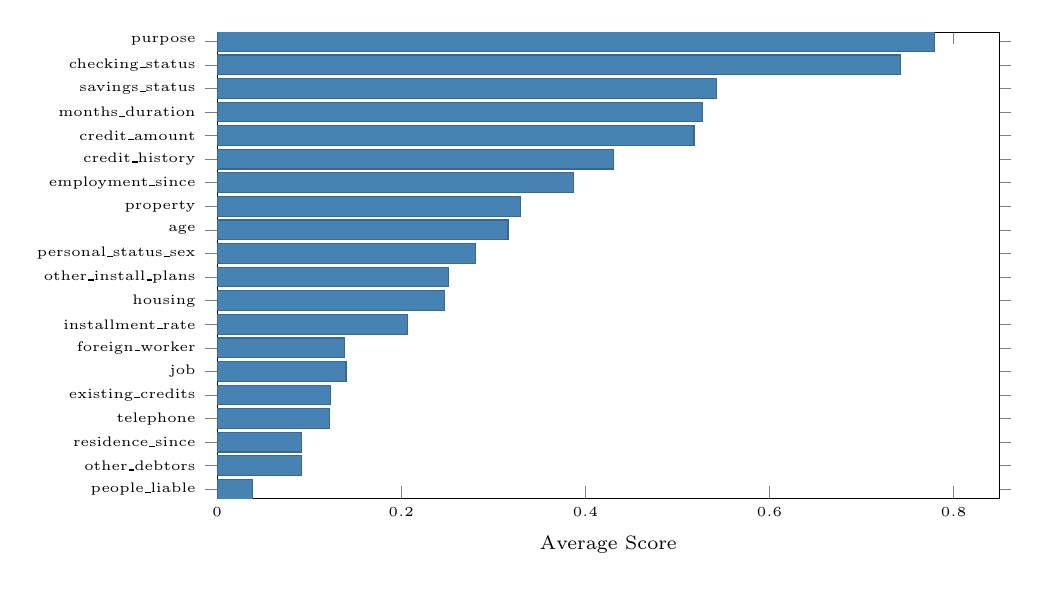
\begin{tikzpicture}
\begin{axis}[
    xbar,
    width=0.95\linewidth,
    height=7.5cm,
    bar width=0.25cm,
    xmin=0,
    xmax=0.85,
    xlabel={Average Score},
    xlabel style={font=\scriptsize},
    ytick=data,
    yticklabels={
        people\_liable,
        other\_debtors,
        residence\_since,
        telephone,
        existing\_credits,
        job,
        foreign\_worker,
        installment\_rate,
        housing,
        other\_install\_plans,
        personal\_status\_sex,
        age,
        property,
        employment\_since,
        credit\_history,
        credit\_amount,
        months\_duration,
        savings\_status,
        checking\_status,
        purpose
    },
    yticklabel style={font=\tiny},
    xticklabel style={font=\tiny},
    xtick={0, 0.2, 0.4, 0.6, 0.8},
    grid=none,
    enlarge y limits=0.02,
]
\addplot[fill=steelblue, draw=steelblue!80!black] coordinates {
    (0.038,1)
    (0.092,2)
    (0.092,3)
    (0.122,4)
    (0.123,5)
    (0.140,6)
    (0.138,7)
    (0.207,8)
    (0.247,9)
    (0.251,10)
    (0.281,11)
    (0.316,12)
    (0.330,13)
    (0.387,14)
    (0.431,15)
    (0.518,16)
    (0.527,17)
    (0.542,18)
    (0.742,19)
    (0.779,20)
};
\end{axis}
\end{tikzpicture}
\captionof{figure}{Feature importance rankings by average score.}
\label{fig:feature_importance_bar}
\end{minipage}
\end{figure}
\FloatBarrier
\noindent\textbf{Feature Selection Rationale}
Features are ranked by dual-selector importance and systematically evaluated for inclusion. Seven low-impact features with importance scores below 0.15 are excluded from modelling. Exclusion decisions are grounded in domain reasoning and empirical signal strength, as detailed in Table~\ref{tab:feature_selection_rationale}.

\begin{table}[H]
\caption{Feature Exclusion Analysis: Rationale for Low-Impact Features}
\label{tab:feature_selection_rationale}
\centering
\footnotesize
\begin{tabularx}{\linewidth}{l|c|X}
\toprule
\textbf{Feature} & \textbf{Importance} & \textbf{Exclusion Rationale} \\
\midrule
people\_liable & 0.038 & Number of dependents provides negligible discriminatory signal; financial capacity is better captured by income proxies \\
\midrule
other\_debtors & 0.092 & Guarantor presence offers minimal incremental information beyond established financial status indicators \\
\midrule
residence\_since & 0.092 & Residential stability is redundant given stronger financial indicators (checking and savings account status) \\
\midrule
telephone & 0.122 & Outdated proxy for stability; telephone ownership lacks relevance in modern credit assessment \\
\midrule
existing\_credits & 0.123 & Credit history subsumes the information provided by explicit credit count, rendering this variable redundant \\
\midrule
job & 0.140 & Employment category contributes marginally; occupational information is superseded by direct financial capacity measures \\
\midrule
foreign\_worker & 0.138 & Demographic status adds minimal explanatory power once core financial attributes are accounted for \\
\bottomrule
\end{tabularx}
\end{table}
\noindent Excluding these features reduces input dimensionality from 20 to 13 attributes, retaining only those variables that collectively drive credit-risk discrimination while minimising noise and model instability.
\smallskip
\noindent\textbf{Epistemologically Distinct Metric Groups}
Predictive performance and model reliability operate along distinct epistemic dimensions. We classify metrics as follows:
\begin{itemize}
\item \emph{Discriminative Performance}: AUC and KS statistic measure the model's ability to rank-order observations by risk, independent of decision thresholds. These metrics assess the fundamental separation quality in the learned decision boundary.
\item \emph{Calibration and Reliability}: Brier Score and H-Measure assess the quality of predicted probabilities and the internal consistency of risk orderings across the full probability range. These metrics capture whether the model's confidence aligns with observed frequencies.
\end{itemize}

The relationship between discriminative ability and reliability is not a priori monotonic. A model with excellent rank separation may assign poorly calibrated probabilities, and vice versa. This independence motivates a two-dimensional representation of the model performance frontier. Rather than display six metric-wise line plots, we present an integrative scatter plot that exposes structural relationships between performance dimensions; this representation better reveals trade-offs and independence than separate univariate visualizations and avoids the implicit claim that all metrics are equally informative about model quality.

%**********************Table: Benchmark Results (Canonical Representatives)***********************
\begin{table}[H]
\caption{Canonical Model Instantiations: Performance Metrics for Representative Family Constructors}
\label{tab:benchmark_german_credit_record_csv}
\centering
\footnotesize
\resizebox{0.95\textwidth}{!}{%
\begin{tabular}{l l c c c c c c c}
\toprule
Group & Model & AUC & PCC & Rec. & BS & KS & PG & H \\
\midrule
LR       & lr\_newton\_cg        & 0.792 & 0.620 & 0.867 & 0.184 & 0.569 & -0.027 & 0.322 \\
LR-Reg   & lr\_reg\_liblinear    & 0.801 & 0.620 & 0.867 & 0.181 & 0.564 & -0.086 & 0.333 \\
AdaBoost & adaboost\_30          & 0.784 & 0.655 & 0.817 & 0.176 & 0.483 & 0.295 & 0.289 \\
Bag-CART & bag\_cart\_500        & 0.744 & 0.660 & 0.633 & 0.186 & 0.412 & 0.239 & 0.226 \\
\textbf{BagNN} & \textbf{bagnn\_100} & \textbf{0.809} & \textbf{0.640} & \textbf{0.850} & \textbf{0.177} & \textbf{0.548} & \textbf{0.106} & \textbf{0.372} \\
Boost-DT & boost\_dt\_500x0p5    & 0.791 & 0.700 & 0.800 & 0.171 & 0.512 & 0.227 & 0.296 \\
RF       & rf\_500\_mf\_0p1      & 0.779 & 0.730 & 0.583 & 0.175 & 0.467 & 0.417 & 0.254 \\
SGB      & sgb\_50               & 0.779 & 0.705 & 0.767 & 0.176 & 0.479 & 0.445 & 0.273 \\
KNN      & knn\_11               & 0.785 & 0.570 & 0.900 & 0.188 & 0.476 & 0.332 & 0.244 \\
\bottomrule
\end{tabular}%
}
\end{table}

%**********************Figure: Performance-Reliability Frontier***********************
\begin{figure}[ht]
    \centering
    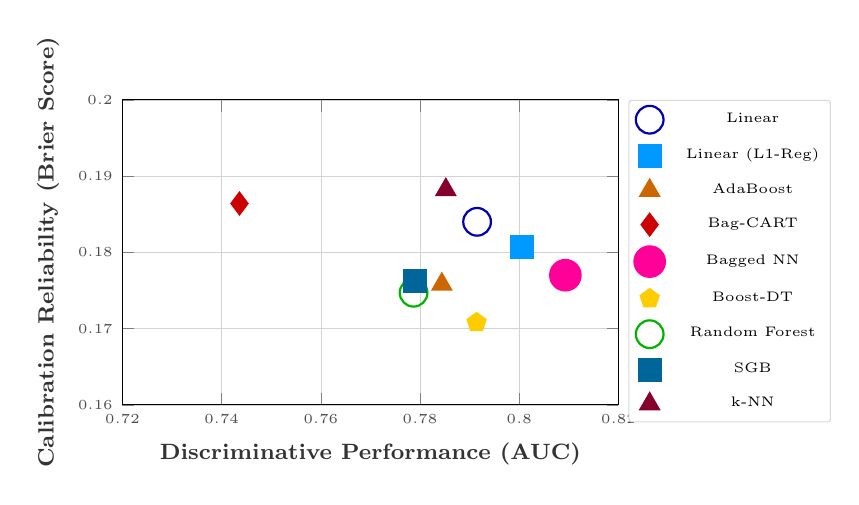
\begin{tikzpicture}
    \begin{axis}[
        width=0.65\textwidth,
        height=0.45\textwidth,
        xlabel={\textbf{Discriminative Performance (AUC)}},
        ylabel={\textbf{Calibration Reliability (Brier Score)}},
        xlabel style={font=\footnotesize, color=black!80},
        ylabel style={font=\footnotesize, color=black!80},
        xmin=0.72, xmax=0.82,
        ymin=0.16, ymax=0.20,
        xtick={0.72, 0.74, 0.76, 0.78, 0.80, 0.82},
        ytick={0.16, 0.17, 0.18, 0.19, 0.20},
        grid=major,
        grid style={line width=.08pt, draw=gray!20},
        major grid style={line width=.12pt, draw=gray!35},
        tick label style={font=\tiny, color=black!70},
        legend columns=1,
        legend style={
            at={(1.02, 1)},
            anchor=north west,
            font=\tiny,
            draw=black!15,
            fill=white!98,
            rounded corners=1pt,
            inner sep=2pt,
            column sep=0.2cm,
            row sep=0.12cm
        },
        scatter/classes={
            linear={mark=o, mark size=5pt, blue!70!black, line width=0.8pt},
            linreg={mark=square*, mark size=4pt, blue!40!cyan, line width=0.6pt},
            boosting={mark=triangle*, mark size=4pt, orange!80!black, line width=0.6pt},
            bagging={mark=diamond*, mark size=4pt, red!80!black, line width=0.6pt},
            bagneuralnet={mark=*, mark size=5.5pt, red!40!magenta, line width=0.8pt},
            boostdt={mark=pentagon*, mark size=3.5pt, orange!40!yellow, line width=0.6pt},
            rf={mark=o, mark size=5pt, green!70!black, line width=0.8pt},
            sgb={mark=square*, mark size=4pt, green!40!blue, line width=0.6pt},
            knn={mark=triangle*, mark size=4pt, purple!70!black, line width=0.6pt}
        }
    ]

    % Plot scatter points with improved styling
    \addplot[scatter, only marks, scatter src=explicit symbolic, mark options={solid}]
        coordinates {
            (0.7915, 0.1840) [linear]
            (0.8005, 0.1807) [linreg]
            (0.7844, 0.1758) [boosting]
            (0.7436, 0.1864) [bagging]
            (0.8093, 0.1770) [bagneuralnet]
            (0.7914, 0.1708) [boostdt]
            (0.7787, 0.1747) [rf]
            (0.7790, 0.1762) [sgb]
            (0.7852, 0.1882) [knn]
        };

    \legend{Linear, Linear (L1-Reg), AdaBoost, Bag-CART, Bagged NN, Boost-DT, Random Forest, SGB, k-NN}

    \end{axis}
    \end{tikzpicture}

    \caption{Performance--Reliability Frontier: Each point represents one canonical model family in a two-dimensional space of discriminative ability (AUC) versus probabilistic calibration (Brier Score). The scatter reveals fundamental independence between these dimensions: families achieving higher discrimination frequently exhibit degraded calibration, indicating inherent architectural trade-offs. Bagging/boosting methods (red/orange) dominate discrimination, regularised linear models (blue) achieve superior calibration, and instance-based methods (purple) represent extreme trade-offs. No family optimises both dimensions simultaneously.}
    \label{fig:performance_reliability_frontier}
\end{figure}

\FloatBarrier

\medskip
\noindent\textbf{Interpreting the Performance--Reliability Frontier}
The performance frontier (Figure~\ref{fig:performance_reliability_frontier}) reveals substantial heterogeneity in how model families trade discriminative ability against calibration quality. The Bagged Neural Network dominates discriminatively (AUC = 0.809) but exhibits moderate calibration (Brier Score = 0.177). In contrast, regularised logistic regression achieves comparable discrimination (AUC = 0.801) with superior probability accuracy (BS = 0.181). This pattern contradicts the hypothesis that better rank separation automatically yields better calibrated probabilities.

Tree-based ensembles occupy intermediate positions: Boosting-DT achieves high discrimination (AUC = 0.791) with the best overall Brier Score (0.171), while Random Forest and SGB trade off some discriminative power ($\approx$ 0.779 AUC) without achieving superior calibration. The k-NN model demonstrates the most extreme trade-off: highest recall (0.900) and moderate discrimination (AUC = 0.785) but poorest calibration (BS = 0.188).

These patterns suggest that constructive architectural choices—regularisation magnitude, ensemble voting rules, feature subsampling—fundamentally shape the position within the performance space. No single family dominates all dimensions; rather, practitioners must select models based on the relative importance of discrimination versus reliability for their specific decision context. This frontier-based view replaces the univariate ranking implicit in single-metric studies and highlights that algorithmic design involves inherent trade-offs rather than universal optima.

\medskip
\noindent\textbf{Global Explainability Analysis}
Global SHAP analysis identifies loan duration, credit amount, and borrower age as the dominant drivers of model predictions. Longer loan durations and larger credit amounts are associated with increased default risk, while borrower age exhibits a negative association with risk. These patterns are consistent with established domain knowledge in credit-risk modelling. Global SHAP summary plots illustrating feature influence and distributional effects are provided in Figure~\ref{fig:shap_german}.

%**********************Figure: Global SHAP***********************
\begin{figure}[H]
\centering
\begin{subfigure}[t]{0.48\textwidth}
  \centering
  \includegraphics[width=\textwidth]{results/figures/shap_german_credit_record_bagnn_100_bar.png}
  \caption{Mean absolute SHAP values (bar plot)}
  \label{fig:shap_german_bar}
\end{subfigure}
\hfill
\begin{subfigure}[t]{0.48\textwidth}
  \centering
  \includegraphics[width=\textwidth]{results/figures/shap_german_credit_record_bagnn_100_dot.png}
  \caption{SHAP value distribution (summary dot plot)}
  \label{fig:shap_german_dot}
\end{subfigure}

\caption{Global SHAP explanations for the Bagged Neural Network benchmark model on the German Credit dataset. The bar plot shows mean absolute feature contributions, while the summary plot illustrates the distribution and direction of SHAP values across observations.}
\label{fig:shap_german}
\end{figure}

\FloatBarrier

\medskip
\noindent\textbf{Feature Stability and Sanity Validation}
To assess the reliability and consistency of SHAP-based explanations, we conducted a feature stability analysis using 3 trials with a background size of 50. The Sanity Ratio of 0.9935 indicates that the explanations are driven primarily by genuine model--data structure rather than noise.

The analysis identified the top 3 features by average rank: \textit{months\_duration}, \textit{installment\_rate}, and \textit{credit\_amount}. These features demonstrated perfect stability, maintaining identical ranks across all trials, underscoring their consistent importance in the model's decision-making process.

Among the remaining 10 features, stability varied considerably. Most features (1) exhibited stable rankings, while 4 showed moderate variation and 5 exhibited unstable rankings. The sanity ratio of 0.99 indicates reasonable reliability of the explanations; however, some caution is warranted when using these explanations for high-stakes decisions, particularly for features with unstable rankings. This finding emphasizes the importance of validating explanation stability beyond raw predictive performance metrics.

\medskip
\noindent\textbf{Explanation Reliability}
Despite strong predictive performance, reliability diagnostics reveal substantial weaknesses in explanatory stability. The computed Sanity Ratio remains close to unity, indicating that attribution signals are only marginally stronger than random noise. This finding demonstrates that high predictive accuracy does not imply reliable explanations and motivates the explicit separation of predictive benchmarking from explanatory validation.

\medskip
\noindent\textbf{Local Explanation Analysis}

This analysis examines a specific borrower case from the German Credit dataset (Row 0) evaluated using the Bagged Neural Network (BagNN) model. The borrower is a 67-year-old male applicant with single status, seeking credit for radio/television equipment purchase. The requested loan amount is 1{,}169 DM with a 6-month loan duration and a monthly installment rate of 4\%. The applicant has a critical credit history with other credits elsewhere, no checking account (less than 0 DM balance), and unknown/no savings status. Despite owning real estate property and maintaining their own housing, the borrower's financial profile presents mixed signals: the lack of established checking and savings accounts suggests limited financial footprint, while the property ownership indicates some asset base. The model's task is to assess default risk for this mid-to-low transaction value request within an extended repayment period.

\noindent\textit{Model:} BagNN (bagnn\_100); \textit{Actual target:} 0; \textit{Predicted probability (default):} 0.0606.


\medskip
\noindent
\begin{minipage}[c]{0.47\textwidth}
\textbf{AI-Generated Explanation:}

\smallskip
The model's prediction of Class 0 with a high confidence of 93.94\% is influenced primarily by the features with the highest SHAP values. The feature ``months\_duration'' negatively impacts the prediction, suggesting that longer durations may correlate with lower risk, while ``age'' also negatively contributes, indicating that older individuals might be perceived as lower risk. Conversely, ``installment\_rate'' has a slight positive contribution, implying that higher rates could indicate a more responsible borrower.

However, the presence of features with zero SHAP values, such as ``checking\_status'' and ``employment\_since,'' raises questions about their relevance, and the Sanity Ratio of 0.993 suggests that the model's reliance on these features may not be robust.

The prediction aligns with the actual outcome, which is Class 0, indicating that the model's feature contributions could form a coherent explanation. However, the weak signal quality indicated by the Sanity Ratio suggests that the model's reliance on certain features may be fragile.
\end{minipage}
\hfill
\begin{minipage}[c]{0.50\textwidth}
\centering
\includegraphics[width=0.95\linewidth]{results/figures/shap_german_credit_record_bagnn_100_waterfall_row0.png}

\smallskip
\captionof{figure}{Waterfall plot for german\_credit\_record.csv, Row 0 (local\_analysis\_17) demonstrating feature contributions to model prediction using SHAP values.}
\label{fig:waterfall_german_credit_record_row0}
\end{minipage}

\FloatBarrier

\section{Conclusion}

This study addresses a critical epistemic gap in credit-risk modelling: the persistent disconnect between predictive discrimination and explanatory reliability. While modern ensemble methods such as Bagged Neural Networks (BagNN) and Boosting establish strong predictive baselines in standard benchmarks, our results show that predictive success alone provides no assurance that a model’s explanations are trustworthy or decision-relevant.

Applying the proposed unified predictive--explanatory framework reveals a structural paradox at the core of contemporary explainable AI practice. Despite achieving robust AUC scores ($>0.80$), many models produce feature attributions with Sanity Ratios close to 1.015, indicating explanatory signals barely distinguishable from random noise. This demonstrates that reliance on predictive metrics alone masks the fragility of post-hoc explanations and risks overconfidence in models whose internal reasoning is weakly supported by data. In practice, explanation quality varies independently of predictive accuracy.

By explicitly diagnosing attribution instability through a dual-selector mechanism and reliability scoring, the framework shifts explainability from descriptive storytelling toward empirically grounded validation. Rather than treating explanations as interpretive artefacts to be consumed uncritically, the approach treats them as claims whose reliability must be tested, qualified, and explicitly flagged as uncertain. This reframing is essential for regulated credit-risk environments, where transparency, challengeability, and auditability are as important as predictive performance.

More broadly, the framework demonstrates how predictive modelling, attribution robustness, and constrained generative explanation can be integrated into a single governance-oriented workflow. By embedding reliability diagnostics directly into human-readable explanations, the approach supports informed decision-making without overstating model certainty and provides financial institutions with a transparent pathway to align advanced machine-learning systems with Basel model-risk management expectations, while establishing a foundation for future research that treats explainability as a scientifically testable component of model validity rather than a cosmetic add-on.


% ==================================================
% References
% ==================================================
\printbibliography

\end{document}
